
\begin{frame} \frametitle{Conclusion}
    \vspace{-.5em}
\begin{block}{Current results}
\begin{itemize}
    \item Higher-order fault injection according to the state of the art 
    \item Positive and negative diagnostic
    \item  A  tool suite based on robust tools (Clang, LLVM, Klee)
\item validation on ``realistic'' applications 
   (PIN verifier, random number generator, OpenSSH, \dots)
\item A  conservative approach for extended fault models
\end{itemize}
\end{block}
    \vspace{.5em}
\vfill

    {\scriptsize ~[PMPD14] Lazart: A symbolic approach for evaluation the robustness of secured codes against control flow injections. In ICST 2014, March 2014.}

    {\scriptsize ~[RPL+14]  Combining High-Level and Low-Level Approaches to Evaluate Software Implementations Robustness Against Multiple Fault Injection Attacks. In FPS 2014, November 2014.}

\end{frame}

\begin{frame} \frametitle{Ongoing work}
\begin{block}{Louis Dureuil's thesis}
\begin{itemize}
\item Higher-order low level fault injection simulator
\item Based on  symbolic execution and static analysis
\item Criteria for guiding physical attacks
\end{itemize}
\end{block}

\vfill
\begin{block}{Project Sertif (Astrid 2014)}
        	\begin{itemize}
\item Simulation pour l'Evaluation de la RobusTesse des applications
embarqu\'ees contre l'Injection de Fautes (V\'erimag, Cesti-Leti, Morpho)

                \item A global process from high-level code analysis to physical attacks
				\item Counter-measure analysis for multiple attacks
                	\item An open-source  benchmark associated with 
evaluation criteria
                	
        	\end{itemize}
\end{block}
\vfill

\end{frame}

\begin{frame}
    \frametitle{Conclusion}
    \begin{center}
        Thanks for your attention!\\
        Question time ?
    \end{center}
\end{frame}

\begin{frame}[fragile]
    \frametitle{Symbolic Execution}
    \begin{columns}[c]
        \column{0.05\textwidth}
        \column{0.5\textwidth}
        \begin{lstlisting}
void foo(int a, int b) {
    make_symbolic(a,b);

    int c = 2*b;
    if (a == 10) {
        if (a >= c) {
            print("Hello");
        }
    }
}
        \end{lstlisting}
        \column{0.45\textwidth}
        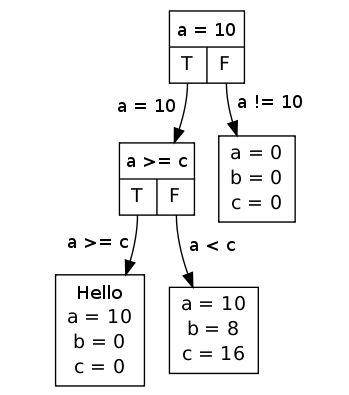
\includegraphics[scale=0.5]{klee_concolic_graph}
    \end{columns}
\end{frame}

\begin{frame} \frametitle{Optionnal mutation operator}
\vfill
%\begin{columns}[t]
%\begin{column}{0.30\textwidth}
%\includegraphics[height=4.5cm]{optional_scheme.pdf} 
\begin{center}
\includegraphics[height=2.5cm]{optional_scheme.pdf}
\end{center}
%\end{column}
%\begin{column}{0.70\textwidth}
\vfill
\begin{center}
\vspace*{-.5cm}
\includegraphics[width=6.5cm]{optional_mutations.pdf}
\end{center} 
%\end{column}
%\end{columns}
\vfill
\end{frame}
